\chapter{PCG for Threshold BBS+}
Most threshold BBS+ schemes (like XXX) necessitate interaction among parties during signing, resulting in communication overhead that leads to latency, especially in scenarios where the signing parties are geographically dispersed. Faust et al. \cite{cryptoeprint:2023/1076} address this limitation with a threshold BBS+ scheme that strategically divides the signing process into two phases: an interactive \textit{offline} preprocessing phase for generating message-independent presignatures and a non-interactive \textit{online} signing phase where presignatures are used without further communication between signers. The essential advantage of this approach is the trade-off it offers. Shifting computationally demanding operations to the offline phase enables a highly efficient online signing process. This flexibility is beneficial for real-world scenarios with variable utilization patterns, allowing presignature generation during low-demand periods to then enable rapid signature creation during peak system load. 
\\\\
We begin by recalling the threshold BBS+ scheme by Faust et al.. We explain how the scheme thresholdizes standard BBS+ to achieve applicability of PCGs, such that their expansion enables the online preprocessing phase. Further, we provide a complete construction for the $n$-out-of-$n$ case then to show the necessary adaption for the $\tau$-out-of-$n$ case. Finally, we implement both cases and provide benchmarks to evaluate the construction.

\section{Thresholdization}
Refer to Definition \ref{definition:bbs+} for the standard BBS+ signature scheme. For simplicity, we focus on the $n$-out-of-$n$ scenario. Therefore, the key generation (\texttt{\textup{KeyGen}}) can be distributed via additive secret sharing. For an $\tau$-out-of-$n$ scenario, Shamir's Secret Sharing  \cite{shamir1979share} (which employs Lagrange interpolation) would be utilized. Notice that for adapting the signing (\texttt{\textup{Sign}}), the main difficulty lies in distributing the computation of Equation \ref{eq:BBS+standardA}.

\begin{equation}
A := \left( g_1\cdot h_0^s\cdot \prod_{\ell \in [k]} h_{\ell}^{m_{\ell}} \right)^{\frac{1}{x+e}}.
\label{eq:BBS+standardA}
\end{equation}

For realizing the non-interactive offline phase, the thresholdization must be able to create message-independent presignatures for $A$ while preventing the disclosure of the secret key (shares of) $x$ during the computation of the inverse of $(x+e)$. This challenge is similar to those faced in other signature schemes that depend on exponentiation, such as ECDSA. Commonly, solving this involves calculating and revealing a value $B = M^a$ and $\delta = a\cdot x$ for a randomly chosen blinding value $a$. The signature of the massage $M^{1/x}$ can then be computed through $B$ without revealing $x$, since $M^{1/x} = B^{1/\delta}$. This is suitable for message-independent presignatures, as $\delta$ remains independent of $M$. This idea is applied in the following.
\\\\
\textbf{BBS+ presignature tuples.} For a $n$-out-of-$n$ setting, secret key $x$, a set of random elements $h_{l \in [0..k]}$ in $\mathbb{G}_1$ and random blinding factor $a$, we define a BBS+ presignature $\varphi_i$ held by party $P_i$ as a tuple $(a_i,e_i,s_i,\delta_i,\alpha_i) \in \mathbb{Z}^5_q$, such that the following correlations hold

\begin{equation}
\begin{array}{l}
\delta=\sum\limits_{i \in[n]} \delta_i=a(x+e), \quad
\sum\limits_{i \in[n]} \alpha_i=as, \\
a=\sum\limits_{i \in[n]} a_i, \quad e=\sum\limits_{i \in[n]} e_i, \quad s=\sum\limits_{i \in[n]} s_i.
\end{array}
\label{eq:req_correlations}
\end{equation}

Assuming the existence of BBS+ presignature tuples $\varphi_i$, we recall the following $n$-out-of-$n$ TSS:

\begin{construction}[\textbf{$n$-out-of-$n$ Threshold BBS+}]
Extending from Construction \ref{definition:bbs+}, let $P_0, \ldots, P_{n-1}$ denote the parties involved, each holding an array of $N$ independent presignatures $\varphi_{i}[1], \ldots, \varphi_{i}[N]$ for party $P_i$. The $n$-out-of-$n$ BBS+ TSS includes the following polynomial-time algorithms:
\begin{itemize}
    \item \texttt{\textup{ThreshKeyGen($1^\lambda$)}}: For a security parameter $\lambda$, sample a secret $x \stackrel{\$}{\leftarrow} \mathbb{Z}_p^*$, compute $y = g_2^x$, and split $x$ as shares ${sk_0, \ldots, sk_{n-1}}$ via a secret sharing scheme. Each party $i$ receives $(pk, sk_i)$.
    \item \texttt{\textup{ThreshSig$_{\varphi_{i}[j]}$($\{m_{\ell}\}_{\ell \in [k]}$)}}: Given secret share $sk_i$ and the \(j\)-th pre-signature $\varphi_{i}[j] = (a_i,e_i,s_i,\delta_i,\alpha_i)$, compute $A_i = h_0^{\alpha_i} \cdot \left( g_1\prod_{\ell \in [k]} h_{\ell}^{m_{\ell}} \right)^{a_i}$ and return partial signature $\sigma_i = (A_i, \delta_i, e_i, s_i)$.
    
    \item \texttt{\textup{CombineSig($\{\sigma_{i}\}_{i \in [n]}$)}}: Combine all partial parital signatures $\{\sigma_{i}\}_{i \in [n]}$ by reconstructing $\delta, e, s$ additively and computing $A = (\prod_{i \in [n]} A_i)^{\frac{1}{\delta}}$ to output $\delta = (A, e, s)$.
    
    \item \texttt{\textup{Verify}}$_{pk}$$(\{m_{\ell}\}_{\ell \in [k]}, \sigma)$: Parse the signature $\sigma = (A, e, s)$ and public key $pk = y$ to output 1 iff $e(A, y \cdot g_2^e) = e(g_1\cdot h_0^s \cdot \prod_{\ell \in [k]} h_{\ell}^{m_{\ell}}, g_2)$.
\end{itemize}
\end{construction}

We observe that \texttt{\textup{CombineSig}} produces a tuple $(A, e, s)$ that represents a valid BBS+ signature as shown in Equation \ref{eq:thresholdBBSplusCorrectness}. Notice that the blinding factor $a$ cancels out. Therefore, the original \texttt{\textup{Verify}} functionality of BBS+ outputs $1$.

\begin{equation}
    A = (\prod_{i \in [n]} A_i)^{\frac{1}{\delta}} = \left( h_0^{as}\cdot (g_1\cdot \prod_{\ell \in [k]} h_{\ell}^{m_{\ell}})^a \right)^{\frac{1}{a(x+e)}} = \left( g_1\cdot h_0^{s}\cdot \prod_{\ell \in [k]} h_{\ell}^{m_{\ell}} \right)^{\frac{1}{x+e}}
\label{eq:thresholdBBSplusCorrectness}  
\end{equation}

Intuitively, the scheme fulfills the \textit{unforgability} property of a TSS (Section \ref{prelim:thresholdSignatures}) as long as no $j$th round of presignatures $\varphi_{0}[j], \ldots, \varphi_{n-1}[j]$ for $j \in [N]$  is used more than once. On the one hand, $a$ and therefore also $\alpha$ and secret $x$ cannot be derived from any (set of) partial signature $\sigma_i$. On the other hand, if each $j$th round of presignatures is independent of any other round $k$ for $k \neq j$ an adversary cannot learn anything from observing valid (partial) signatures.

\section{Online Preprocessing Phase}
We recalled the construction of a non-interactive $n$-out-of-$n$ BBS+ TSS from \cite{cryptoeprint:2023/1076}, assuming the existence of a message-independent presignature database that satisfies two criteria: (1) each set of presignatures satisfies the specified correlations (cf. Equation \ref{eq:req_correlations}), and (2) each set is computationally indistinguishable from all others so that forgery of unused (partial) presignatures is not possible. These are attributes a PCG (Definition \ref{def:PCGprelim}) can fulfill, as it can securely produce pseudorandom distributions that are correlated in some pre-defined way. Criteria (1) follows from the PCGs \textit{correctness} property, and criteria (2) from the PCGs \textit{security} property.
\\\\
\textbf{Correlations.} Notice that the correlations of BBS+ tuples can be decomposed into two OLE and one VOLE correlation. Specifically, the correlation $\alpha = as$ can be realized as an OLE correlation by assuming that $a$ and $s$ are already additively shared among the parties. Each party $i$, for $i, j \in [n]$, then receives shares of the cross-terms $a_is_j$ (for $i \neq j$) represented as  $a_is_j = z_{(i,j)}^i+z_{(i,j)}^j$. Here, $z_{(i,j)}^i$ denotes the share held by party $i$ and $z_{(i,j)}^j$ denotes the share held by party $j$. Note that party $i$ can compute the term $a_is_i$ locally. Finally, each party $i$ can construct its additive share of $\alpha = \sum_{i\in [n]}\alpha_i$ as in Equation \ref{eq:additiveShareAlpha}:

\begin{equation}
  \alpha_i=a_is_i + \sum_{j \in [n]\backslash \{i\}}{z_{(i,j)}^i} + \sum_{j \in [n]\backslash \{i\}}z_{(j,i)}^i.
  \label{eq:additiveShareAlpha}
\end{equation}

This also works for the other correlations. Notice, that $\delta = a(x+e)$ can be split into an OLE correlation $\delta^0 = ae$ and a VOLE correlation $\delta^1 = ax$, where the secret $x$ is invariant, allowing us to express $\delta$ as the sum $\delta = \delta^0 + \delta^1$. Since there are no other requirements, we can utilize the PCG constructions for (V)OLE correlations introduced in Section \ref{sec:construction} to construct a PCG for BBS+ tuples.

\subsection{PCG Construction for BBS+}
The basic idea behind combining the (V)OLE constructions of Section \ref{sec:construction} for connecting multiple correlations is that we let the individual PCG instantiations share LPN error vectors strategically. Simultaneously, the LPN error vectors themselves can be utilized as additive shares of $a$, $e$, and $s$. We present the PCG construction for BBS+ tuples (Equation \ref{eq:req_correlations}) in Construction \ref{construction:PCGforBBS+}.
\\\\
\textbf{Seed Generation.} For PCG.Gen$_{\texttt{BBS+}}$, we begin with sampling additive secret key shares $sk_i$. We also sample LPN error vectors for every party. Each set of error vectors represents a seed for an additive share of the targeted base parameter $a \sim (\boldsymbol{\omega}, \boldsymbol{\beta})$, $e \sim (\boldsymbol{\eta}, \boldsymbol{\gamma})$, $s \sim (\boldsymbol{\phi}, \boldsymbol{\epsilon})$. In step 3, we initiate the VOLE PCG, for which $sk_i$ serves as the constant parameter. Notice that we multiply the $j$th parties secret share $sk_j$ with $\boldsymbol{\beta}_i$ as we realize a secret share for all cross-term $a_i\cdot sk_j$. For $a_i\cdot sk_i$ a distribution is unnecessary as party $i$ holds all necessary parts. In step 4, we initiate the PCG for OLE for all cross-terms. Notice here how the LPN error vectors of $a$, $(\boldsymbol{\omega}, \boldsymbol{\beta})$ are used for both initiations. This embeds to the relation of the correlations ($\delta_0 = a\cdot e$ and $\alpha = a\cdot s$) the individual PCGs can be expanded for. Ultimately, the seeds that include the party's respective secret key share, the LPN error vectors, and the DSPF keys are returned.
\\\\
\textbf{Seed Expansion.} For PCG.Expand$_{\texttt{BBS+}}$, we begin by reconstructing the LPN error polynomials from the seed. In step 2, each party computes its share of the VOLE correlation by adding its known adjacent term with all shares of the cross-terms. Notice that both directions of the cross-terms need to be evaluated from the DSPF. Similarly, in step 3, the OLE correlations are being evaluated. All parameters are then interpreted as vectors of polynomials. Analogusly to the PCG construction for (V)OLE, computing the inner product of those polynomials with public parameter $a$, then yields ring elements in $R_p$ that adheres to the specified correlations. In order to extract individual BBS+ pairs in $\mathbb{Z}_{p}$, the ring elements need to be split via evaluation on a common root of unity as described in Section \ref{subseq:realtiontofx}.

\begin{specialconstruction}{PCG for BBS+ Tuples}
\label{construction:PCGforBBS+}
\vspace{1em}

Let $\lambda$ be the security parameter, $(t,c)$ the parameters of the $R^c$-LPN$_t$ assumption, and $p$ the modulus. We denote $N$ as the domain of the PCG. Further, let $R_p:=\mathbb{Z}_{p}[X]/(F(X))$ be a ring for a degree $N$ polynomial $F(X) \in \mathbb{Z}_{p}[X]$ and $\boldsymbol{a} = (1, a_2, ..., a_c)$ for $a_2, ...,a_c \in R_p$ be a public input.

\vspace{1em}

\textbf{PCG.Gen$_{\texttt{BBS+}}(1^\lambda)$:}

\begin{algorithmic}[1]
\State Sample key shares $\mathrm{sk}_{i} \stackrel{\$}{\leftarrow} \mathbb{Z}_{p}$ for every $i \in [n]$.
\State For every $i \in [n], r \in [c]$, sample $\boldsymbol{\omega}_{i}^{r}, \boldsymbol{\eta}_{i}^{r}, \boldsymbol{\phi}_{i}^{r} \stackrel{\$}{\leftarrow} [N]^{t}$ and $\boldsymbol{\beta}_{i}^{r}, \boldsymbol{\gamma}_{i}^{r}, \boldsymbol{\epsilon}_{i}^{r} \stackrel{\$}{\leftarrow} [\mathbb{Z}_{p}]^{t}$ uniformly at random.
\State For every $i, j \in [n]$ with $i \neq j, r \in [c]$, compute
\begin{align*}
& \left(U_{i, j}^{r, 0}, U_{i, j}^{r, 1}\right) \stackrel{\$}{\leftarrow} \texttt{DSPF}_{N}^{t}.\texttt{Gen}\left(\mathbbm{1}^{\lambda}, \boldsymbol{\omega}_{i}^{r}, \mathrm{sk}_{j} \cdot \boldsymbol{\beta}_{i}^{r}\right).
\end{align*}
\State For every $i, j \in [n]$ with $i \neq j, r, s \in [c]$, compute
\begin{align*}
& \left(C_{i, j}^{r, s, 0}, C_{i, j}^{r, s, 1}\right)\stackrel{\$}{\leftarrow} \texttt{DSPF}_{2N}^{t^{2}}.\texttt{Gen}\left(\mathbbm{1}^{\lambda}, \boldsymbol{\omega}_{i}^{r} \boxplus \boldsymbol{\eta}_{j}^{s}, \boldsymbol{\beta}_{i}^{r} \otimes \boldsymbol{\gamma}_{j}^{s}\right), \\
& \left(V_{i, j}^{r, s, 0}, V_{i, j}^{r, s, 1}\right) \stackrel{\$}{\leftarrow} \texttt{DSPF}_{2N}^{t^{2}}.\texttt{Gen}\left(\mathbbm{1}^{\lambda}, \boldsymbol{\omega}_{i}^{r} \boxplus \boldsymbol{\phi}_{j}^{s}, \boldsymbol{\beta}_{i}^{r} \otimes \boldsymbol{\epsilon}_{j}^{s}\right).
\end{align*}
\State For every $i \in [n]$, output the seed
\begin{align*}
\kappa_{i} \leftarrow\left(\mathrm{sk}_{i},\left(\boldsymbol{\omega}_{i}^{r}, \boldsymbol{\eta}_{i}^{r}, \boldsymbol{\phi}_{i}^{r}\right)_{r \in [c]},\left(\boldsymbol{\beta}_{i}^{r}, \boldsymbol{\gamma}_{i}^{r}, \boldsymbol{\epsilon}_{i}^{r}\right)_{r \in [c]},\left(U_{i, j}^{r, 0}, U_{j, i}^{r, 1}, C_{i, j}^{r, s, 0}, C_{j, i}^{r, s, 1}, V_{i, j}^{r, s, 0}, V_{j, i}^{r, s, 1}\right)_{\substack{j \neq i \\ r, s \in [c]}}\right).
\end{align*}
\end{algorithmic}

\vspace{1em} % Space before the next part

\textbf{PCG.Expand$_{\texttt{BBS+}}(\sigma, \kappa_\sigma)$:}

\begin{algorithmic}[1]
\State For every $r \in [c]$, define the degree $< N$, $t$-sparse LPN polynomials:
\begin{align*}
u_{i}^{r}(X):= \sum_{l \in [t]} \beta_{i}^{r}[l] \cdot X^{\omega_{i}^{r}[l]}, \quad  v_{i}^{r}(X):= \sum_{l \in [t]} \gamma_{i}^{r}[l] \cdot X^{\eta_{i}^{r}[l]}, \quad  k_{i}^{r}(X):= \sum_{l \in [t]} \epsilon_{i}^{r}[l] \cdot X^{\phi_{i}^{r}[l]}.
\end{align*}
\State For every $r \in [c]$, compute:
\begin{align*}
& \widetilde{u}_{i}^{r} \leftarrow \mathrm{sk}_{i} \cdot u_{i}^{r}+\sum_{j \neq i}\left(\texttt{DSPF}_{N}^{t}.\texttt{FullEval}\left(U_{i, j}^{r, 0}\right)+\texttt{DSPF}_{N}^{t}.\texttt{FullEval}\left(U_{j, i}^{r, 1}\right)\right).
\end{align*}

\State For every $r, s \in [c]$, compute
\begin{align*}
& w_{i}^{r, s} \leftarrow u_{i}^{r} \cdot v_{i}^{s}+\sum_{j \neq i}\left(\texttt{DSPF}_{2N}^{t^{2}}.\texttt{FullEval}\left(C_{i, j}^{r, s, 0}\right)+\texttt{DSPF}_{2N}^{t^{2}}.\texttt{FullEval}\left(C_{j, i}^{r, s, 1}\right)\right), \\
& m_{i}^{r, s} \leftarrow u_{i}^{r} \cdot k_{i}^{s}+\sum_{j \neq i}\left(\texttt{DSPF}_{2N}^{t^{2}}.\texttt{FullEval}\left(V_{i, j}^{r, s, 0}\right)+\texttt{DSPF}_{2N}^{t^{2}}.\texttt{FullEval}\left(V_{j, i}^{r, s, 1}\right)\right).
\end{align*}

\State Define the vectors of polynomials $\boldsymbol{u}_{i} := (u_{i}^{0}, \ldots, u_{i}^{c-1})$, and similarly for $\boldsymbol{v}_{i}$, $\boldsymbol{k}_{i}$, and $\widetilde{\boldsymbol{u}}_{i}$.

\State Let $\boldsymbol{w}_{i} := (w_{i}^{0,0}, \ldots, w_{i}^{c-1,0}, w_{i}^{0,1}, \ldots, w_{i}^{c-1,1}, \ldots, w_{i}^{c-1, c-1})$, and similarly for $\boldsymbol{m}_{i}$.

\State Compute the final polynomials
\begin{align*}
a_{i} & \leftarrow \left\langle\boldsymbol{a}, \boldsymbol{u}_{i}\right\rangle, & 
s_{i} & \leftarrow \left\langle\boldsymbol{a}, \boldsymbol{v}_{i}\right\rangle, &
e_{i} & \leftarrow \left\langle\boldsymbol{a}, \boldsymbol{k}_{i}\right\rangle, \\
\alpha_{i} & \leftarrow \left\langle\boldsymbol{a} \otimes \boldsymbol{a},  \boldsymbol{w}_{i}\right\rangle, & 
\delta_{i}^{0} & \leftarrow \left\langle\boldsymbol{a} \otimes \boldsymbol{a},  \boldsymbol{m}_{i}\right\rangle, & 
\delta_{i}^{1} & \leftarrow \left\langle\boldsymbol{a},  \widetilde{\boldsymbol{u}}_{i}\right\rangle, \\
& & & & \delta_{i} & \leftarrow \delta_{i}^{0} + \delta_{i}^{1}
\end{align*}
in $\mathbb{F}_{q}[X] / (F(X))$. Output $\left(\alpha_{i}, \mathrm{sk}_{i}, a_{i}, s_{i}, e_{i}, \delta_{i}\right)$.
\end{algorithmic}
\end{specialconstruction}



\subsubsection{Complexity}
Although the BBS+ tuples only contain two OLE and one VOLE correlation, the presented PCG primitives for (V)OLE (Section X) realize these correlations for two parties. Therefore, Construction X would need to instantiate significantly more primitives for additional parties; each new party requires additional cross-terms. Naively, for $n$ parties, the PCG for BBS+ would consist of $n^2-1$ individual VOLE PCGs and $2\cdot(n^2-1)$ OLE PCGs. This suggests a potentially quadratic scaling. However, notice that Construction X intertwines the individual primitives. Recall from Section X that generating ring elements (step 6) dominates the runtime, especially for large $N$. By directly summing the full domain evaluations, we mitigate this step to generate only five ring elements, independent of the number of parties ($n$). Since ring element generation involves the superlinear FFT while full domain evaluations are linear, our construction's overall complexity remains superlinear with respect to the domain size $N$. For $n$ on the other hand, we notice that each additional party adds six full domain evaluations (step 2/3) to the expansion. Therefore, Construction X computational complexity is superlinear for domain $N$, and linear for the participating parties $n$. Section X provides a detailed evaluation of these claims.

\subsection{$\tau$-out-of-$n$ setting}
In particular, the summation of the full domain evaluations in step 2/3 hinders compatibility with a $\tau$-out-of-$n$ setting, for $\tau < n$. In this setting, parties require only specific cross-term subsets determined by the current signer set. Direct summation prevents this selective use. Furthermore, summing all cross-terms together impedes interpolation on secret key shares when employing methods like Shamir's Secret Sharing \cite{shamir1979share}.  
\\\\
\textbf{Solution.} We can solve this by individually computing the full domain evaluations and generating a ring element (via $a$) for each. This allows parties to evaluate only the needed ring elements and subsequently interpolate the secret shares according to the signer set. Finally, they can combine all parts to obtain a valid BBS+ tuple. Note that each full domain evaluation must be stored individually for the VOLE component (step 2). However, the forward and backward evaluations can be summed directly in the OLE case (step 3) since interpolation isn't required there. This solution does come with drawbacks. First, there is increased storage overhead since all intermediate results (in form or additional ring elements) need to be retained. Second, computational overhead arises during the expansion due to the need of generating significantly more ring elements (one for each cross-term). We analyze the severity of these computational drawbacks in the following section. Note that, depending on the signer set, the ring elements can be recombined before being split. Therefore, there is no overhead at this point, except for a few (negligible) additions determined by $\tau$. Otherwise, $\tau$ has no influence on the complexity of this appraoch.

\section{Evaluation}
In this section we are going to evaluate our implementation of the PCG for Threshold BBS+ described above. We start with the $n$-out-of-$n$ setting and compare it's performance over different amounts of parties $n$ and domain choices $N$. Further, we evaluate our implementation of the $\tau$-out-of-$n$ setting. We validate, that both settings stay superlinear (regarding $N$) driven through the use of FFT for generating the ring elements and that an increase in parties only comes with an linear increase in runtime. We conclude, that this behavior implies that the use of this PCG for Threshold BBS+ in order to realize an online pre-processing phase to enable an efficient non-interactive offline signing phase is practical. 
\\\\
\textbf{Setup.} We reuse the setup of Chapter \ref{chapter:evaluation}, with the same optimizations and parallelization of the building blocks in place. Because of the complexity of the benchmarks and the large number of repetitions within the constructions, we only execute the benchmark for each parameter selection once.

\subsection{$n$-out-of-$n$}
We evaluate our implementation of the $n$-out-of-$n$ setting for parties $n\in \{2, ..., 10\}$ and domains $N\in \{2^{11}, ...,2^{19}\}$ in Figure \ref{fig:BBSnoutofn}. As expected, we observe a superlinear runtime increase with respect to the domain size $N$ for all party counts. Concurrently, runtime increases linearly as the number of parties ($n$). This aligns with our complexity analysis:

\begin{itemize}
    \item \textbf{Ring Element Generation:} Independent from $n$, while contributing a superlinear runtime increase for $N$ due the use of FFT.
    \item \textbf{Full Domain Evaluations:} Instantiations scale with $n$, while their linear $O(N)$ complexity (cf. Section X) aligns with the observed linear increase with respect to party count.
\end{itemize}

Compared to the original OLE PCG (Figure X), our BBS+ construction achieves a disproportionately favorable runtime, even though it handles multiple correlations (2 OLE, 1 VOLE). Focusing on the two-party case for a fair comparison, a single BBS+ tuple requires 100ms at $N=17$, while a single OLE correlation takes roughly 60ms. This highlights the effectiveness of intertwining the PCG primitives.

\subsection{$\tau$-out-of-$n$}
We evaluate our implementation of the $\tau$-out-of-$n$ setting for $\tau = 2$, parties $n\in \{3, ..., 10\}$ and domains $N\in \{2^{11}, ...,2^{18}\}$ in Figure \ref{fig:BBSnoutofn}. We observe again, that the runtime increases superlinear for domain $N$. In contrast to the $n$-out-of-$n$ setting before, the runtime increase over $N$ is notably steeper. This behavior derives from the fact that the construction now needs to deal with more ring elements, leading to more frequent use of FFT. Since FFT is used more frequently, the primitive has a higher (non-linear) impact on the total runtime. 
\\\\
Directly comparing runtimes, we find the $\tau$-out-of-$n$ implementation takes roughly 37\% longer for $N=17$ and $n=3$, with similar differences existing for other values of $n$. This confirms that the presented adaption for realizing the $\tau$-out-of-$n$ setting, while introducing some overhead, remains computationally manageable.

\subsection{Identifying Bottlenecks}
Recall that in individual (V)OLE constructions, generating ring elements using FFT was the primary performance bottleneck, especially for large domains. However, let's analyze how this changes within the context of the BBS+ PCG. Figure \ref{fig:runtimeAllocationComparision} breaks down the construction's runtime for different party counts ($n$) on $N=17$.
\\\\
In the $\tau$-out-of-$n$ setting, the proportion of time spent on full domain evaluations versus ring element generation remains roughly constant. The reason for this is that as $n$ becomes larger, more full domain evaluations are needed for each of which additional ring elements need to be created. Therefore the runtime allocation is close to constant for this case. Interestingly, in the $n$-out-of-$n$ setting, ring element generation becomes less dominant. This trend is expected, as the number of ring elements stays fixed while full domain evaluations increase with $n$.  Surprisingly, in contrast to FFT being costly within the individual (V)OLE PCG, our analysis reveals that full domain evaluations of DSPFs represent the primary bottleneck in the BBS+ PCG. Therefore, we determine that further optimizing this building block would significantly improve the overall construction's performance.

\subsection{Implications on the TSS scheme}
We notice that the presented benchmarks show the apllicablity of a PCG for this BBS+ scheme.
implementation benefits Blablabla. The results are blabla.  

\textbf{Overhead in the Offline Phase}
% Idea: For the tau out of n case, we cannot split the ring on all roots of unity AS we need the singing set for this. Therefore this step adds to the offline phase and needs to be performed during signing. This brings additional overhead.

\textbf{Comparison with [].}


\begin{figure}[t]
    \centering
    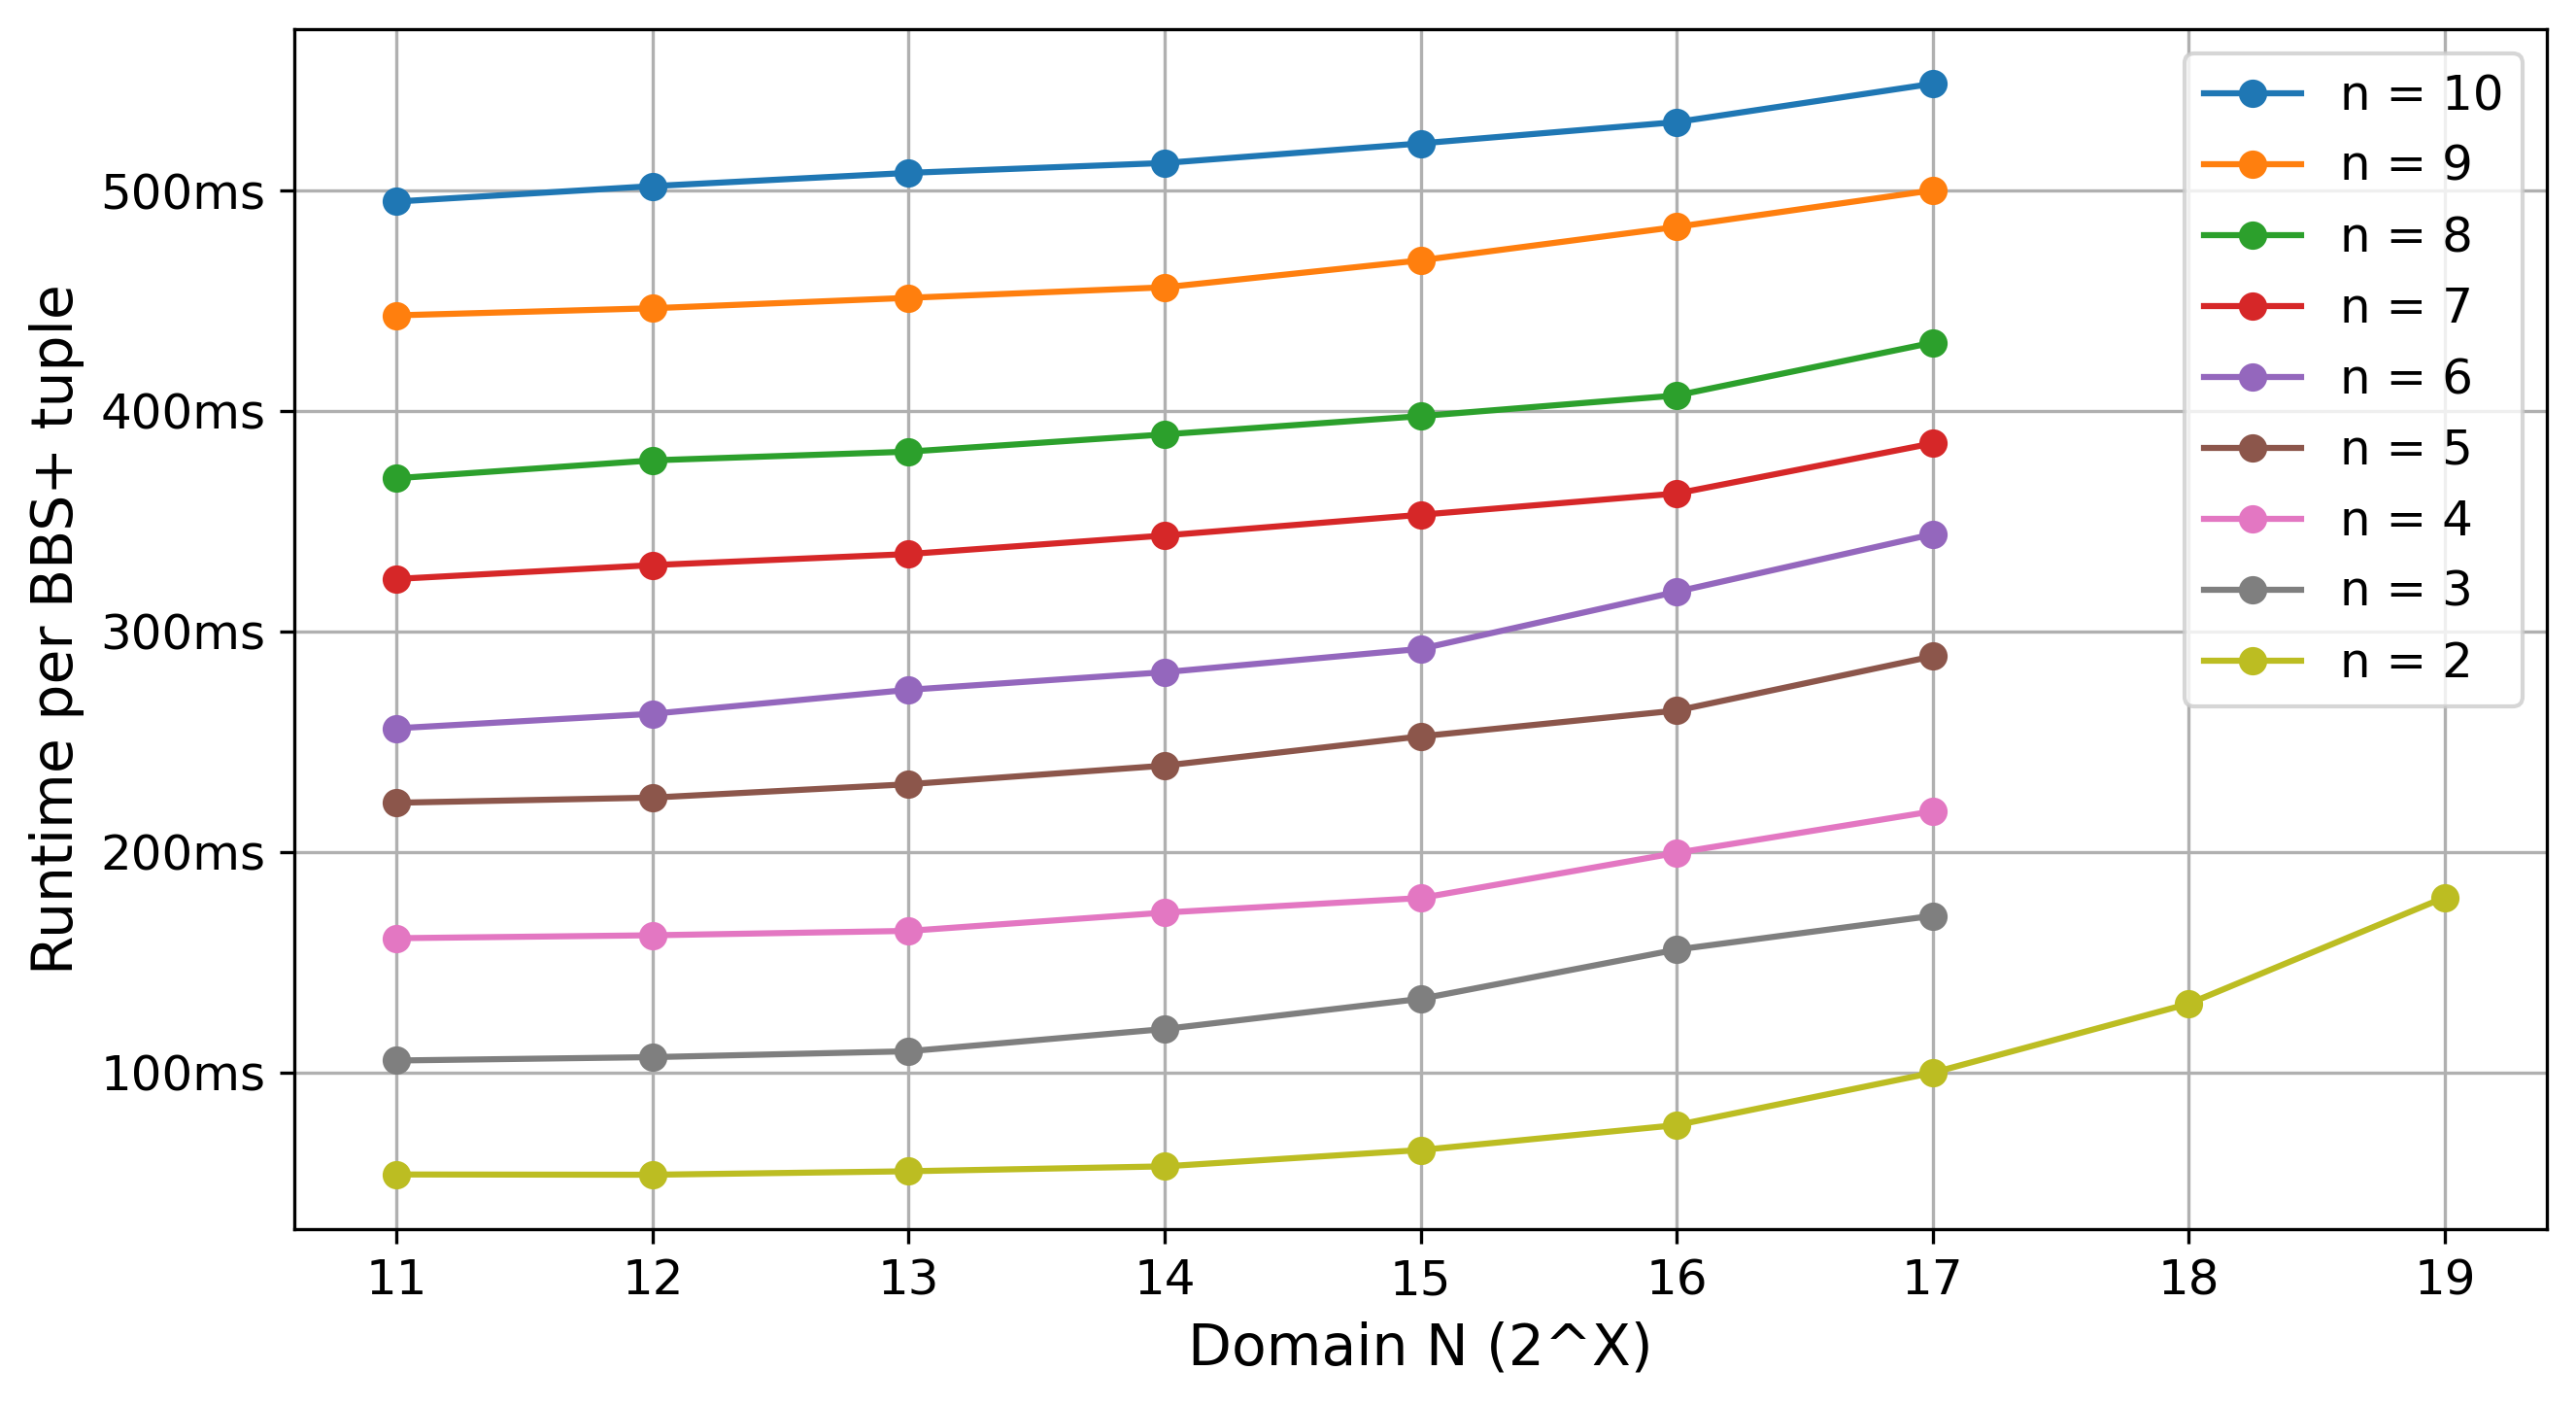
\includegraphics[scale=0.49]{images/plots/bbs_pcg_NoutofN.png}
    \caption{$n$-out-of-$n$ BBS+ PCG expansion over $N$}
    \label{fig:BBSnoutofn}
\end{figure}

\begin{figure}[t]
    \centering
    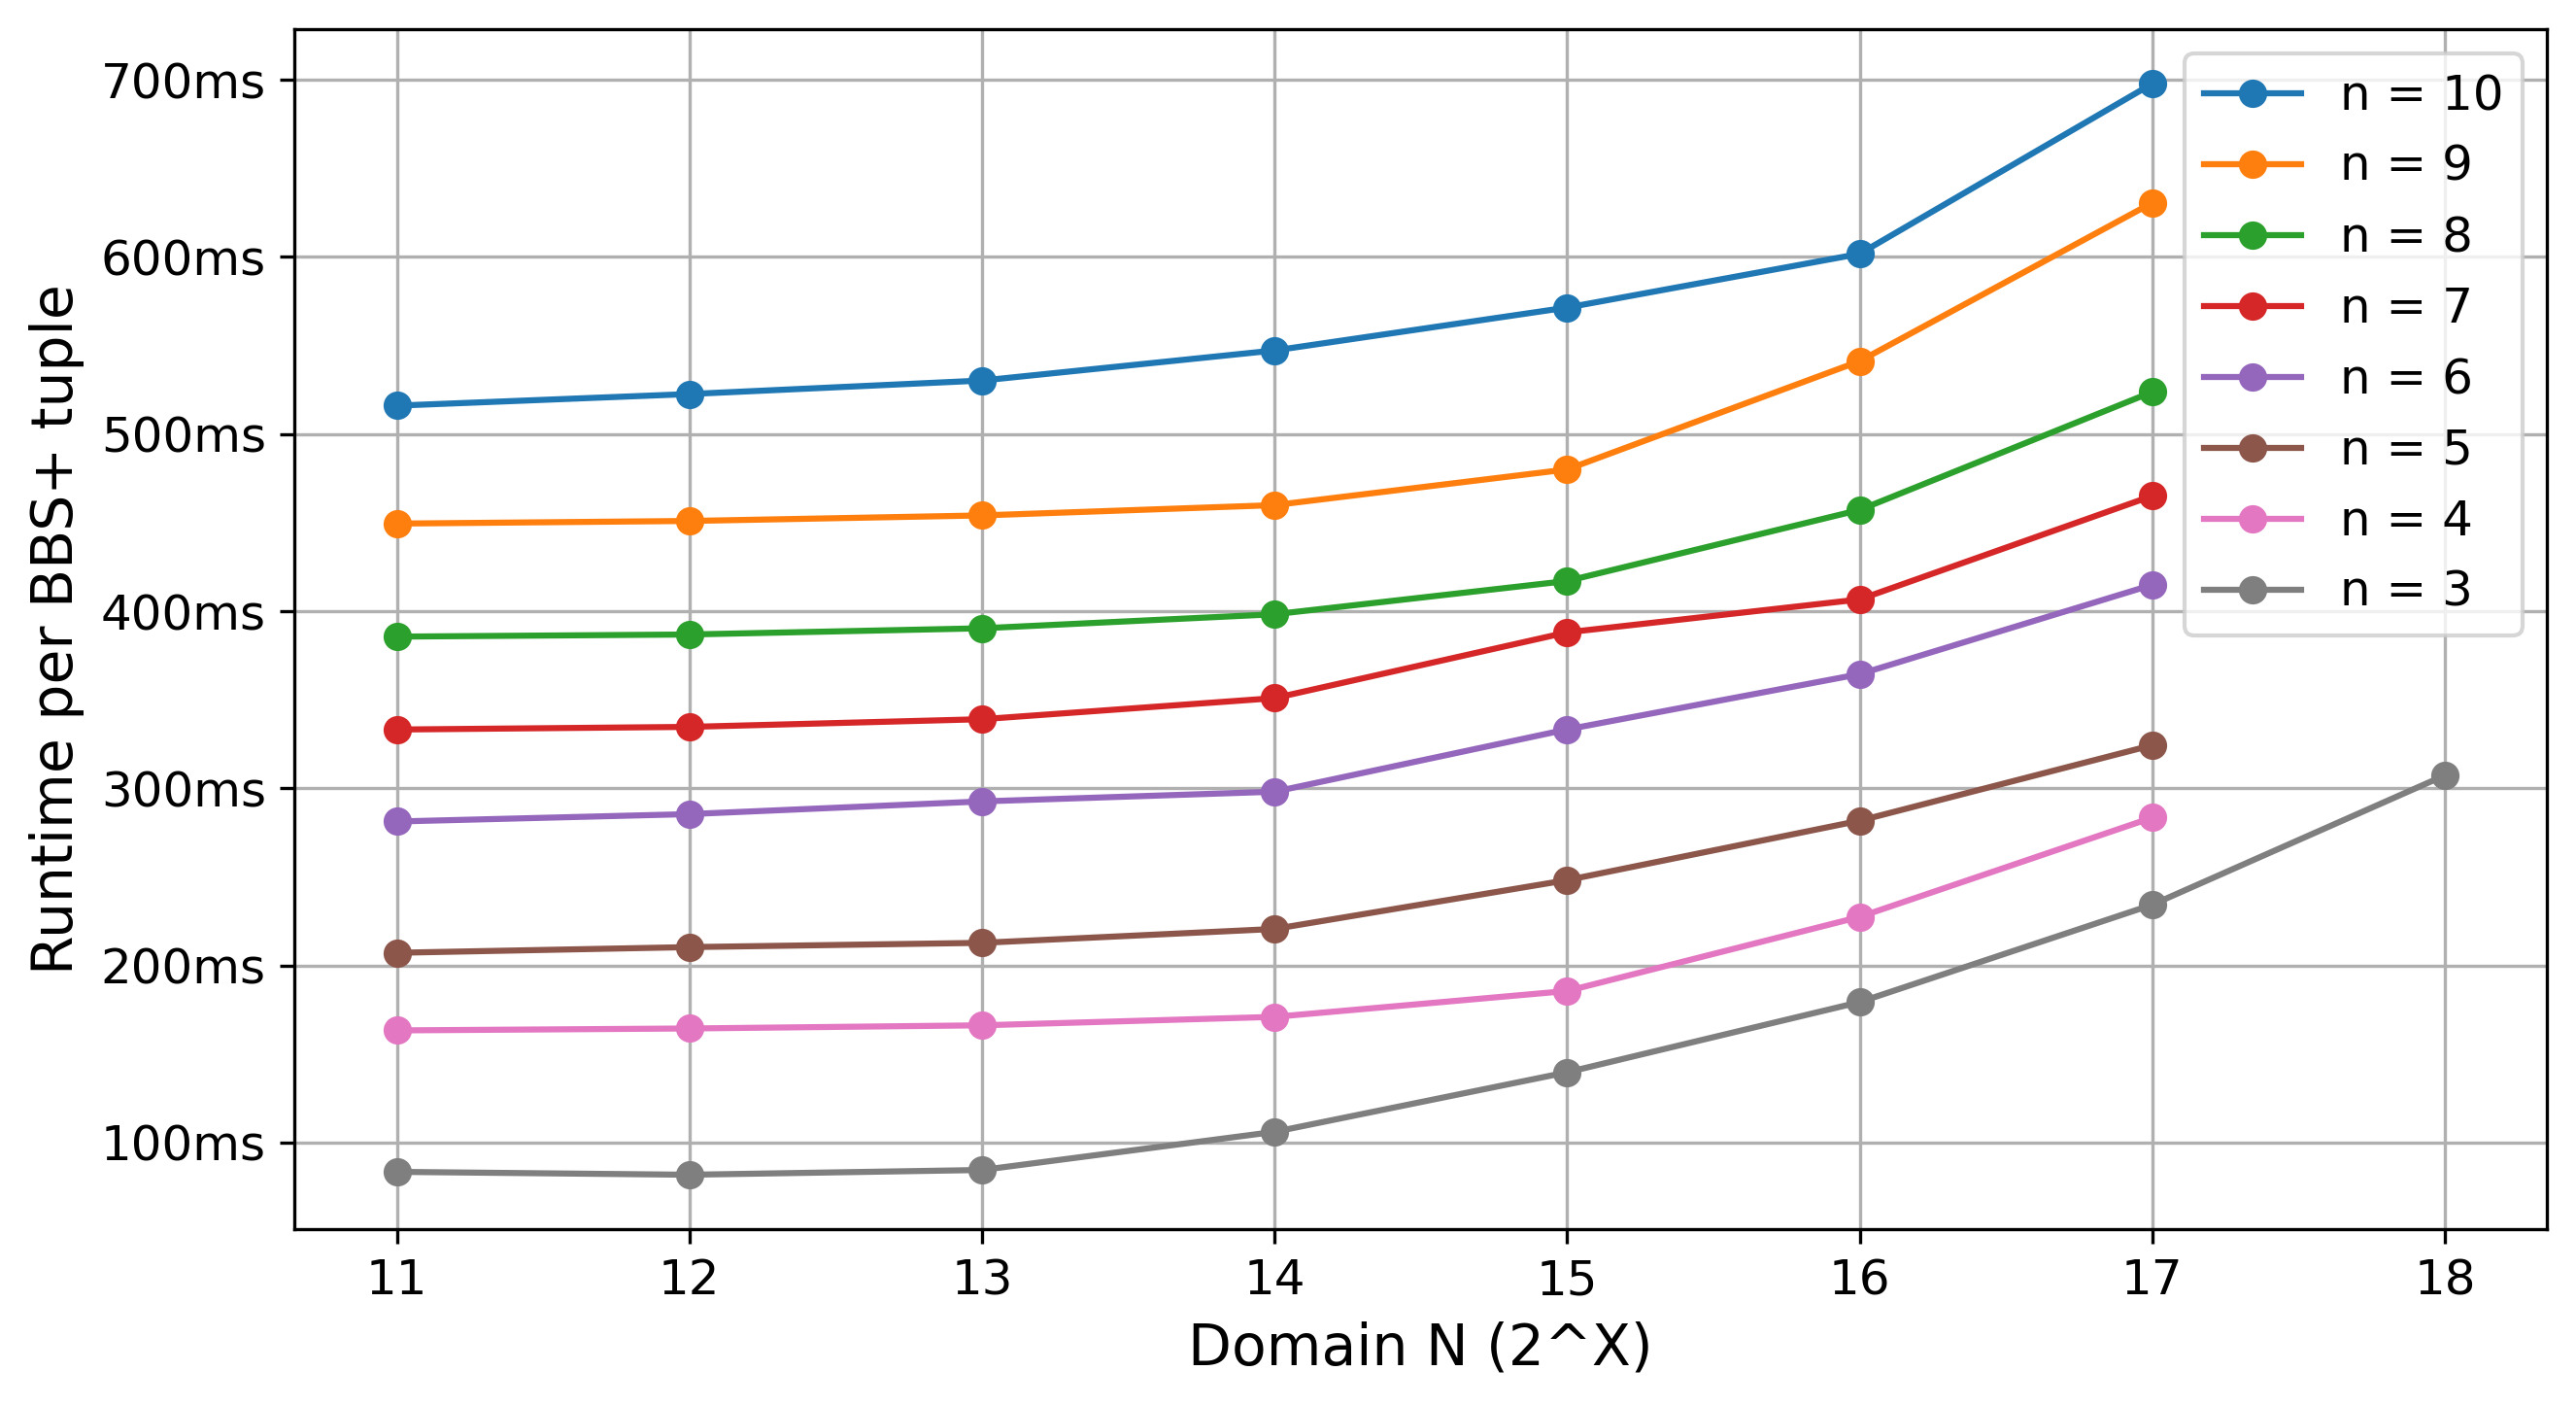
\includegraphics[scale=0.49]{images/plots/bbs_pcg_TAUoutofN.png}
    \caption{$2$-out-of-$n$ BBS+ PCG expansion over $N$}
    \label{fig:BBStauoutofn}
\end{figure}

\begin{figure}[t]
    %\centering
    \hspace{-1em}
    \begin{subfigure}[b]{0.5\textwidth}
        \centering
        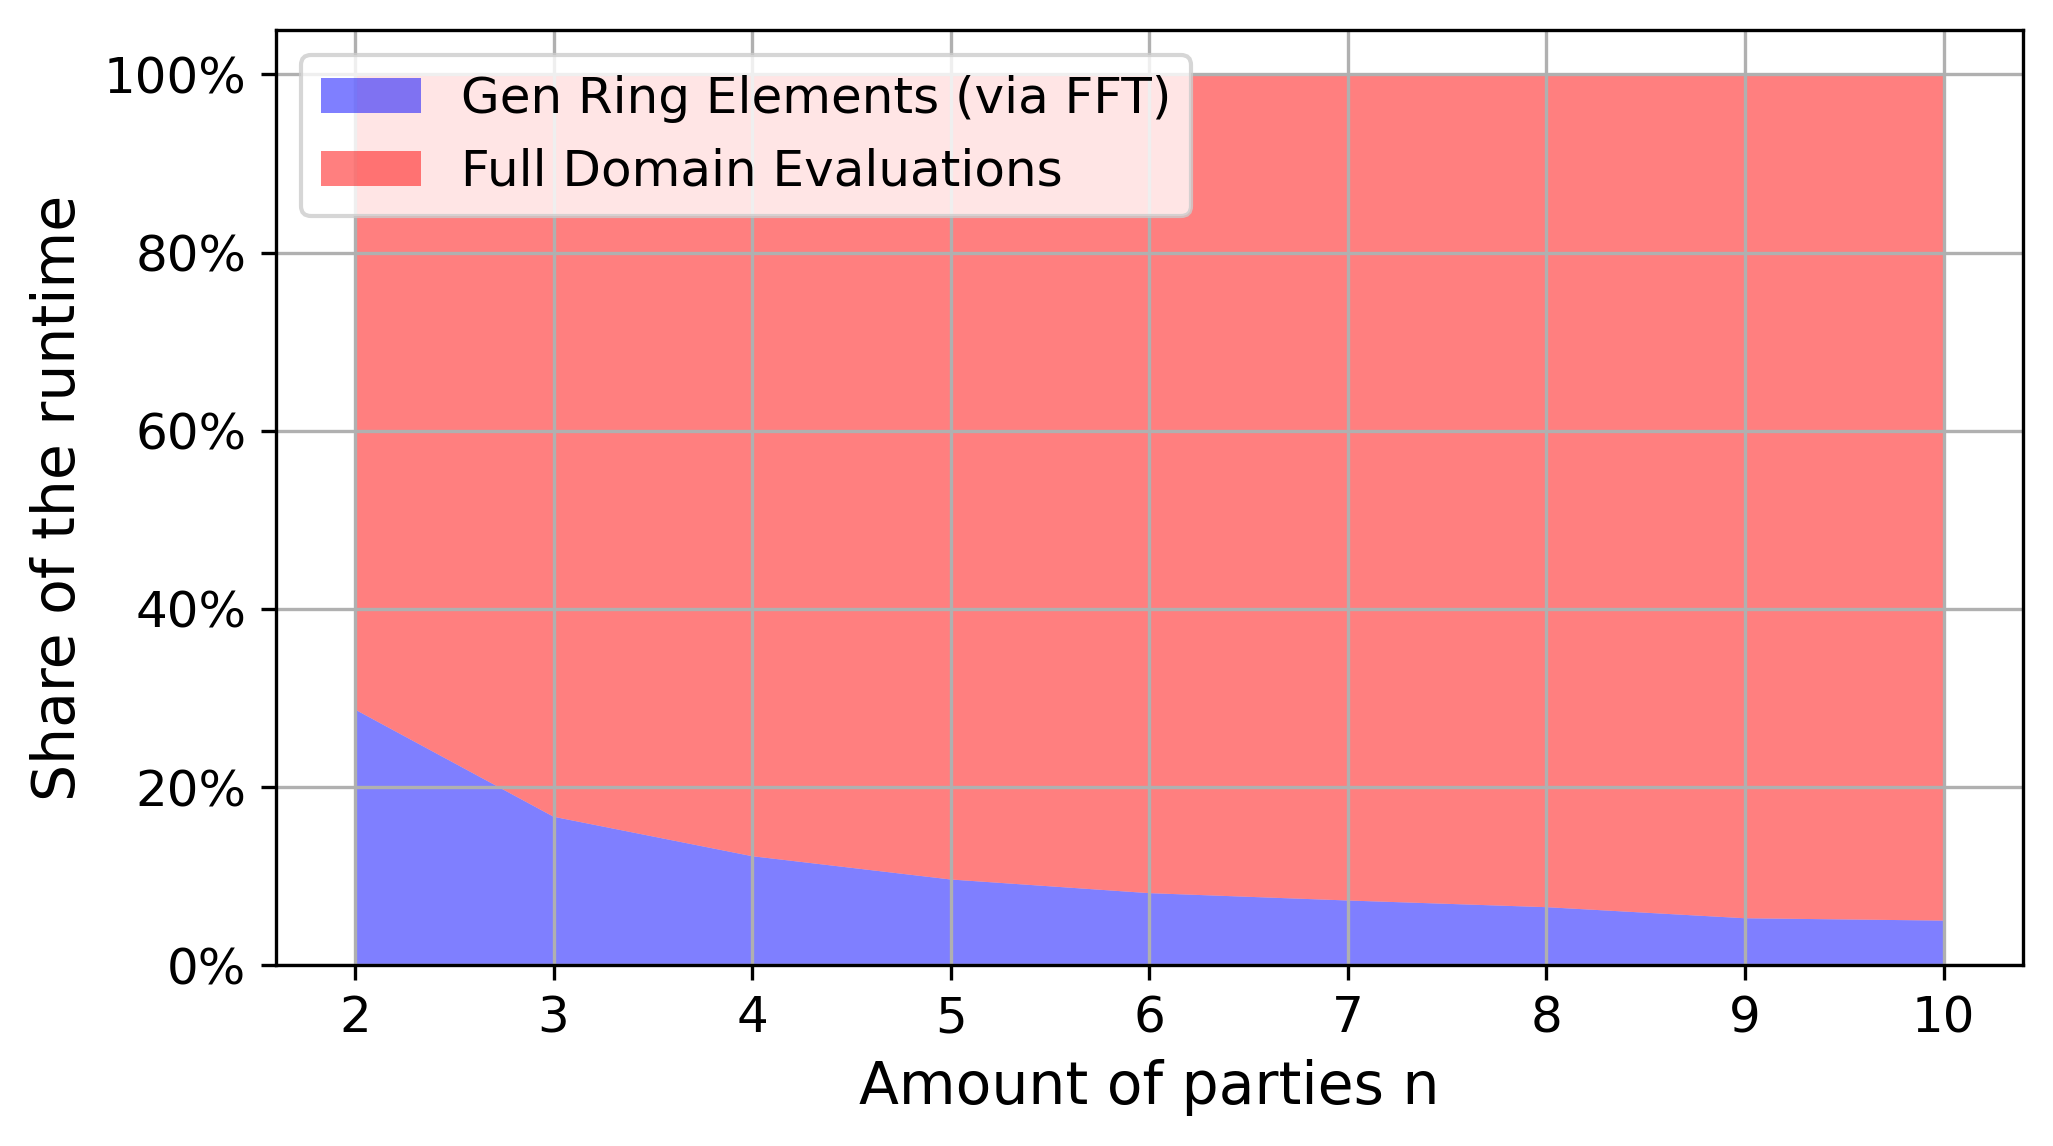
\includegraphics[scale=0.49]{images/plots/bbs_noutofN_percentage_dist.png}
        \caption{$n$-out-of-$n$}
    \end{subfigure}
    \hspace{0em}
    \begin{subfigure}[b]{0.5\textwidth}
        \centering
        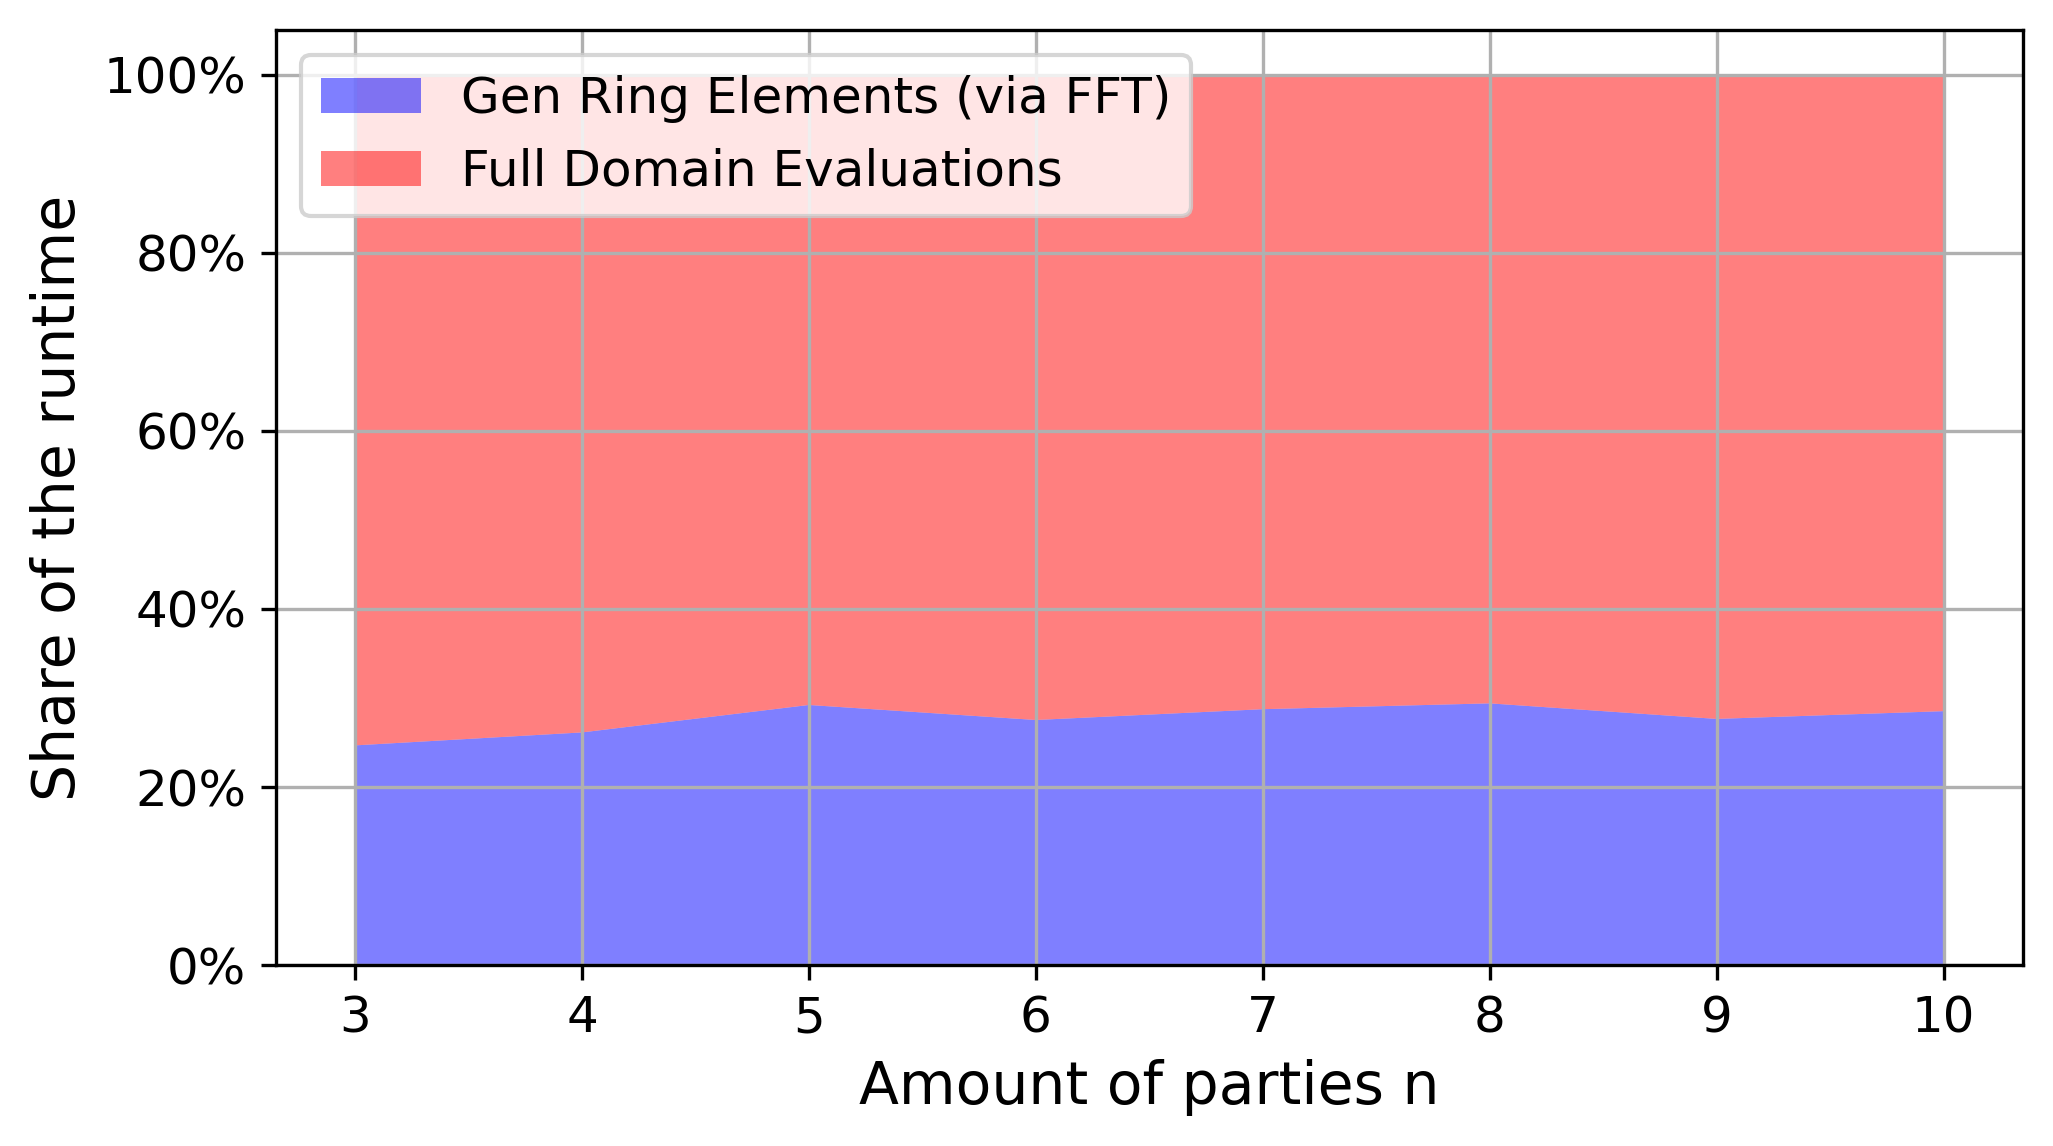
\includegraphics[scale=0.49]{images/plots/bbs_TAUoutofN_percentage_dist.png}
        \caption{$2$-out-of-$n$}
    \end{subfigure}
    \label{fig:runtimeAllocationComparision}
    \caption{Comparing runtime allocation of $n$-out-of-$n$ with $2$-out-of-$n$ for $N=17$}
\end{figure}
